\providecommand{\main}{..}
\documentclass[\main/main.tex]{subfiles}
\begin{document}

\chapter{The classifier}

\section{Training the classifier}

\subsection{Convert documents to vector representation}
Given a set of training class-labeled elements \(T\), we convert the documents, treated as \textit{bag of elements}, to enumeration-sorted frequency vectors.

Given a document composed of \(n=\#d\) elements \(d = \crl{e_1, e_2, \ldots, e_n}\), first we define \(d_\neq \subseteq d\) as the set of distinct elements in \(d\). Then, we map to every distinct element its normalized cardinality in the set \(d\):
\[
	z(e_i) = \frac{\arity{e_j \in d: e_j=e_i}}{n}
\]
Then, we proceed to map to a common enumeration the elements, using as full-set of elements the entire training set elements, so that \(\forall e_i, e_j \in T, \exists! i, j \in \N: i=j \Leftrightarrow e_i=e_j \).

\subsection{Choosing representative points}
Given an arbitrary percentage of points \(p \in \sqr{0,1}\) and an arbitrary distance in percentage \(\alpha \in \sqr{0,1}\), for each class of points \(C_j \in T\) we choose using \(k\)-Means:
\[
	k=\ceil{\#C_j\cdot p^2}
\]
This way the centroids surely distribute among the different points, following their density. If the points are, in truth, a unique cluster, the centroids will distribute themselves in an uniform fashion.

Then, we select following a random uniform distribution for each cluster \(Q_i \in \crl{Q_1, \ldots, Q_k}\) a number \(\floor{\arity{p \in C_j: p \in Q_i}\cdot p}\) points. We move each point \(p\) of an amount proportional to the distance from the point to its centroid \(c_i\):\(\alpha \cdot L^2\rnd{p, c_i}\) towards its centroid.

\subsubsection{Using a metric to choose k}
For the high dimensionality and number of the vectors, iterating multiple times \textit{KMeans} searching for an optimal \(k\) following any given metric has an high time cost. For this reason, an attempt using \textbf{PCA} to reduce the dimensionality and predict the number of clusters in high dimensionality space using a density metric was made.

\paragraph*{The density was defined as follows:}
\[
	\bar{\rho}_{jk} = \frac{1}{k} \sum_{i=1}^k \rho_{{jk}_i} = \frac{1}{k} \sum_{i=1}^k \rnd{\frac{\arity{\bmv \in C_{r_j}:\bmv \in Q_i}}{\#C_{r_j}}}^k \cdot \frac{1}{r_{Q_i}^2} \qquad r_{Q_i}^2 = \begin{cases}
		\frac{1}{n} \sum_{h=1}^{n} {(\bmc_i - \bmp_h)}^2 & \text{if \(n \neq 0\)} \\
		1                                                & \text{else}
	\end{cases}
\]
Where \(r_{Q_i}\) is the approximated radius of the cluster \(Qk_i\), using the farthest \(n\) frontier points \(p_f\).

\paragraph*{Does the prediction hold?}
While the metric on two dimensions reduction seemed to work, when iterated on increasingly larger number of dimensions, with the exception of strongly clustered data, it did not much better than a random selection.

As follows, with 2D PCA density metrics the heuristic seems to be successful to identify the number of clusters \(k\) necessary to describe the given classes.
\begin{figure}
	\begin{subfigure}{0.24\textwidth}
		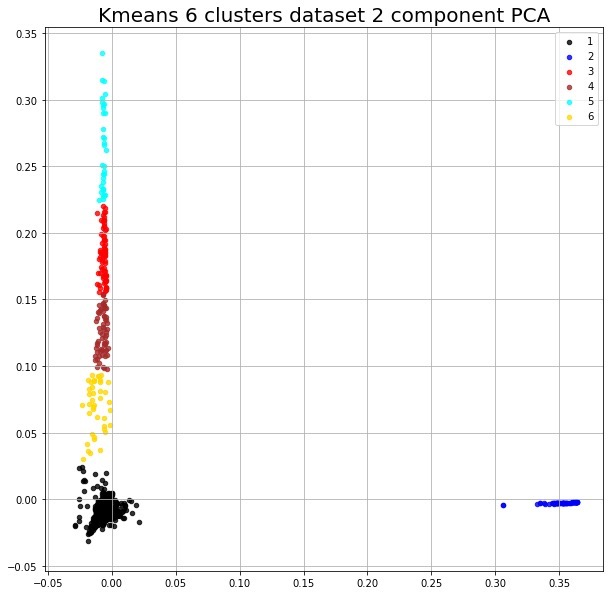
\includegraphics[width=\textwidth]{multi-cluster}
		\caption{Data with multi-clusters, 2D PCA, \(k=6\)}
	\end{subfigure}
	~
	\begin{subfigure}{0.24\textwidth}
		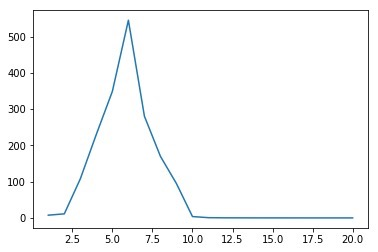
\includegraphics[width=\textwidth]{multi-cluster-pca-score}
		\caption{Density for data multi-clusters, 2D PCA, density/k}
	\end{subfigure}
	~
	\begin{subfigure}{0.24\textwidth}
		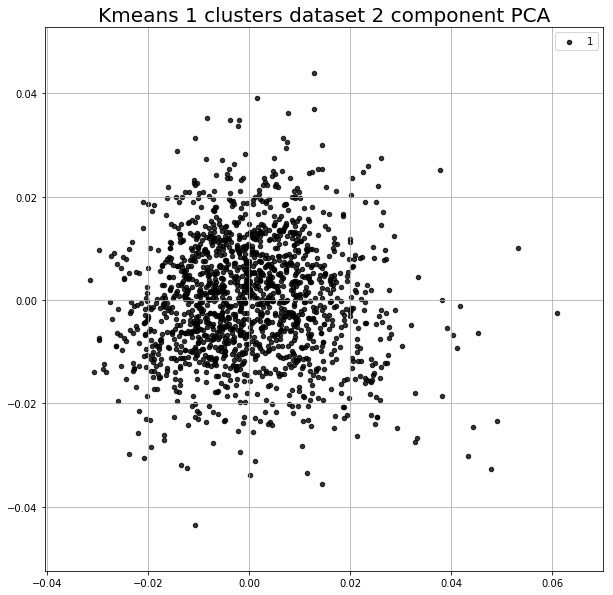
\includegraphics[width=\textwidth]{one-cluster}
		\caption{Data with single-cluster, 2D PCA, \(k=1\)}
	\end{subfigure}
	~
	\begin{subfigure}{0.24\textwidth}
		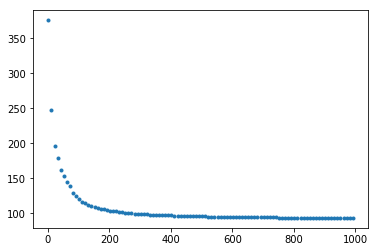
\includegraphics[width=\textwidth]{one-cluster-pca}
		\caption{Density for data single-cluster, 2D PCA, density/k}
	\end{subfigure}
\end{figure}

The prediction on any given PCA reduction however is not valid for different dimension numbers, on multi-clusters classes.

Any number of clusters \(k\) high enough (\(k>5\)) is no more precise than a density metric. With increasing number of clusters, as shown below, it becomes increasingly unreliable.

\begin{figure}
	\begin{subfigure}{0.49\textwidth}
		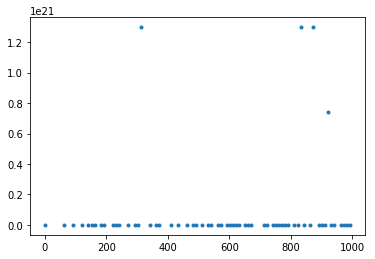
\includegraphics[width=\textwidth]{one-cluster-pca-k}
		\caption{Best value of \(k\) for increasing dimensions in PCA reduction, one-clusters data.}
	\end{subfigure}
	~
	\begin{subfigure}{0.49\textwidth}
		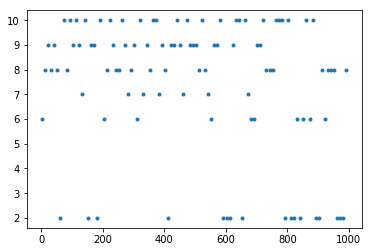
\includegraphics[width=\textwidth]{multi-cluster-pca-k}
		\caption{Best value of \(k\) for increasing dimensions in PCA reduction, multi-clusters data.}
	\end{subfigure}
\end{figure}

\subsection{Completing the classifier}
The classifier model is now finished, comprised of every class-labeled representative point.


\section{Classifying a document}
To classify a given a document \(d\) we proceed as follows:
\begin{enumerate}
	\item Convert the document \(d\) to a zipf representative vector, using the common enumeration: \(\bmv = z(d)\).
	\item The document is then classified with the same label as the closest representative point in the classifier model.
\end{enumerate}


\end{document}